\customHeader{1}{\BERT{} Models for \textclassification}
\label{02_bert_models_for_text_classification}

A \emph{Language Model} is a \neuralNetwork{} that can be used for predicting the distribution of tokens, given a corpus. The main goal of a Language Model is to capture the underlying patterns and structure of tokens in the corpus.
The architecture for the \gls{bert} (Bidirectional Encoder Representations from Transformers) family of models was introduced \mytextcite{BERT_paper} as one capable of learning embeddings aware of the left and right context for each token\footnote{Hence the name ``Bidirectional".}. 
\putInBox{
The \BERT{} family of models has gained significant popularity due to its ability to efficiently generate contextualized embeddings for both individual tokens and entire documents at a low cost \myparencite{revolution_bert}.
}
While the original \gls{bert} is a general-purpose model, many tasks benefit from domain-specific knowledge. The multitude of \gls{bert} models arises from the need to cater to different languages, domains, tasks, and computational constraints, combined with ongoing research efforts to improve model performance and efficiency. 

Many \gls{bert} models are freely and readily accessible and set for deployment across a range of \gls{nlp} tasks. Given this availability, they will serve as primary tools for this work.



\customHeader{2}{Attention and Transformers}
\label{02_attention_and_transformers}


For many years, \gls{nlp} methods faced challenges with understanding distant relationships within texts. For example, consider the sentence, ``The cat, which was adopted from the shelter last month, loves to play.". Here, the subject (cat) and the verb (loves) are spaced apart by several words, making it tricky for systems identifying grammatical roles. Similarly, when translating from, say, Japanese to English, it's crucial to recognize that the Japanese verb typically appears at the end of the sentence. 

Initially introduced in \gls{nlp} for Machine Translation \myparencite{attention_for_translation}, the \emph{Attention} mechanism enables the \neuralNetwork{} to focus on particular words or phrases crucial for grasping the context. 
It achieves this by employing trainable parameters to determine coefficients between 0 and 1, indicating the significance of each input token to each output token (Figure \ref{fig:02_attention_for_translation}). The part of the network responsible for determining these attention coefficients is termed an \emph{Attention Head}.

Interestingly, attention can be computed between a sentence and itself to evaluate the significance of its various components relative to one another; this process is called \emph{Self-Attention}. The outcome of the Self-Attention mechanism for a text comprising $n$ tokens is an $n\times n$ matrix $A=(a_{ij})$, where $a_ij$ is a value between 0 and 1, denoting the influence of token $j$ on token $i$ (typically, $p_{ij}\neq p_{ji}$). In the original architecture, which we employ in this work, the time and memory usage for Self-Attention grow in a quadratic manner on the text's length ($O(n^2)$). More recent Self-Attention designs aim to reduce computing time \cite{flash_attention}.


\begin{figure}
    \centering
    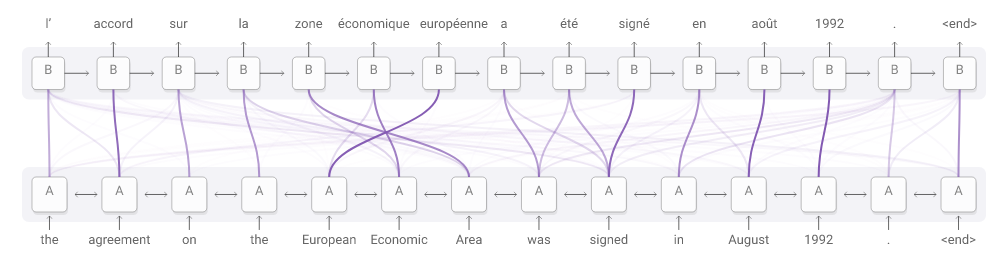
\includegraphics[width=.75\textwidth]{Figures/02/Attention_for_translation.png}
    \caption{Attention Mechanism for Machine Translation, from \mytextcite{attention_distilled}}
    \label{fig:02_attention_for_translation}
\end{figure}


Attention mechanisms are a fundamental component of \emph{Transformer} models, a type of deep learning architecture that has revolutionized \gls{nlp} tasks. The original Transformer model, introduced in the ``Attention is All You Need" paper by \cite{attention_is_all_you_need}, uses multiple a Self-Attention Heads, and is primarily used for sequence-to-sequence tasks, such as Machine Translation.

A classical Transformer architecture consists of two main neural modules, the \emph{Encoder} and the \emph{Decoder}. The encoder module takes embeddings as input features, computes self-attention, and produces attention-enriched embeddings.
These enhanced embeddings are then channeled to the decoder, which outputs the logits of the probabilities of the next token.
Notably, the decoder also incorporates its prior outputs as inputs, applies self-attention to them, and then calculates "cross" attention between these and the attention-augmented embeddings from the encoder. The design of this architecture is depicted in Figure \ref{fig:02_transformer_architecture}.

After successful training, the encoder learns the optimal way to generate embeddings for each token considering all the other tokens in the input. At the same time, the decoder learns to produce tokens in a manner informed by the input and its own output. Due to the quadratic complexity of Self-Attention, Transformer architectures have a limited input size.


\begin{figure}
    \centering
    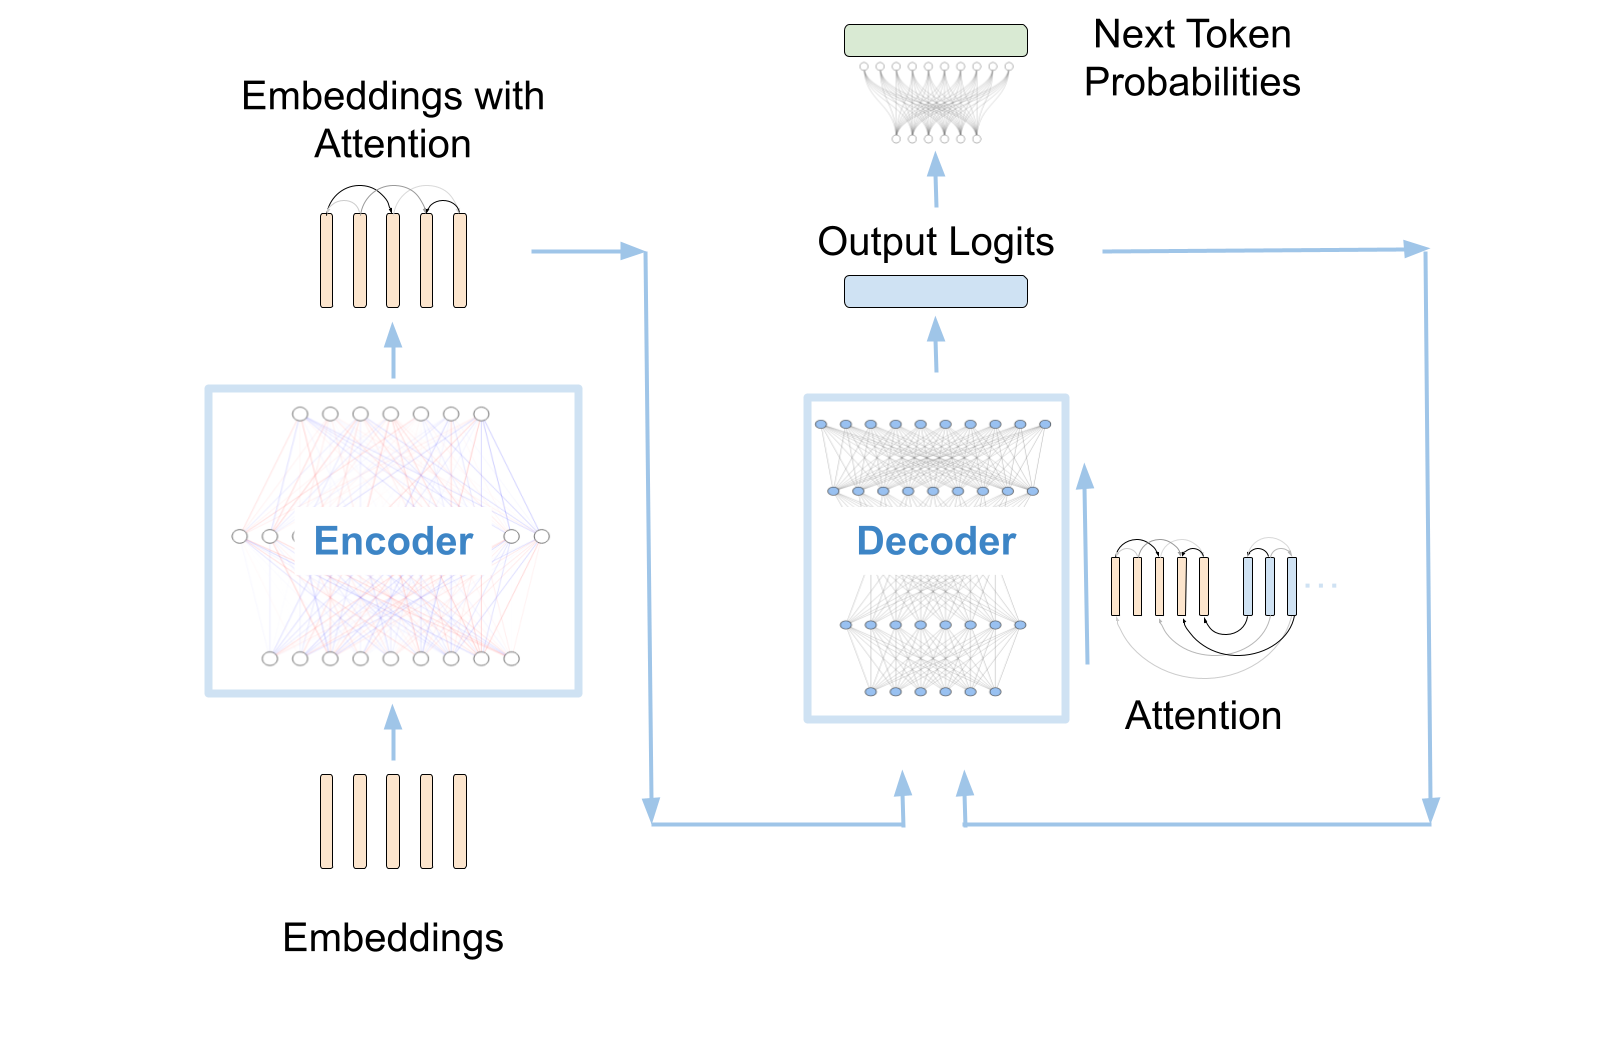
\includegraphics[width=0.75\textwidth]{Figures/02/02_transformer.png}
    \caption{Classical Transformer Architecture}
    \label{fig:02_transformer_architecture}
\end{figure}







\customHeader{2}{The training of \BERT{}}
\label{02_training_bert}

The architecture for \gls{bert}  essentially a series of encoder modules from the traditional Transformer design, layered sequentially\footnote{Hence the name ``Encoder Representations from Transformers".}. 
Two distinct versions were introduced by the original auhors for English text: a base model with 12 encoder layers and 12 attention heads, yielding 768-dimensional embeddings, and a large model with 24 encoder layers and 16 attention heads, resulting in 1024-dimensional embeddings. The basic \gls{bert} architecture employs a \gls{wp} tokenizer and can handle up to 512 tokens as input.

For training \gls{bert} to generate context-aware embeddings for individual tokens as well as entire sentences, it was subjected to two specific tasks. The datasets utilized for this purpose were Google's BookCorpus and the English portion of Wikipedia.

\customHeader{3}{Masked Language Modeling}
\label{02_mlm}

To learn embeddings for tokens, the authors introduce the \gls{mlm} task.
At its core, the \gls{mlm} task aims for the model to ``fill-in the blank" or to ``guess the missing word". For \gls{mlm}, once a text is tokenized, 15\% of the tokens are randomly substituted with a unique \texttt{[MASK]} token, symbolizing a blank space. This modified sequence is then processed by the encoder layers, relying on the self-attention mechanisms to provide sufficient contextual understanding (as depicted in Figure \ref{fig:02_attention_mlm}). To determine the omitted word, the final embedding corresponding to the \texttt{[MASK]} token is passed through a \gls{softmax} activation function, yielding a probability distribution over all the tokens in the vocabulary. By contrasting these probabilities with the known token, the cross-entropy loss is computed, which serves as the loss to be minimized. This procedure enables \gls{bert} to learn about the token distribution.



\begin{figure}
    \centering
    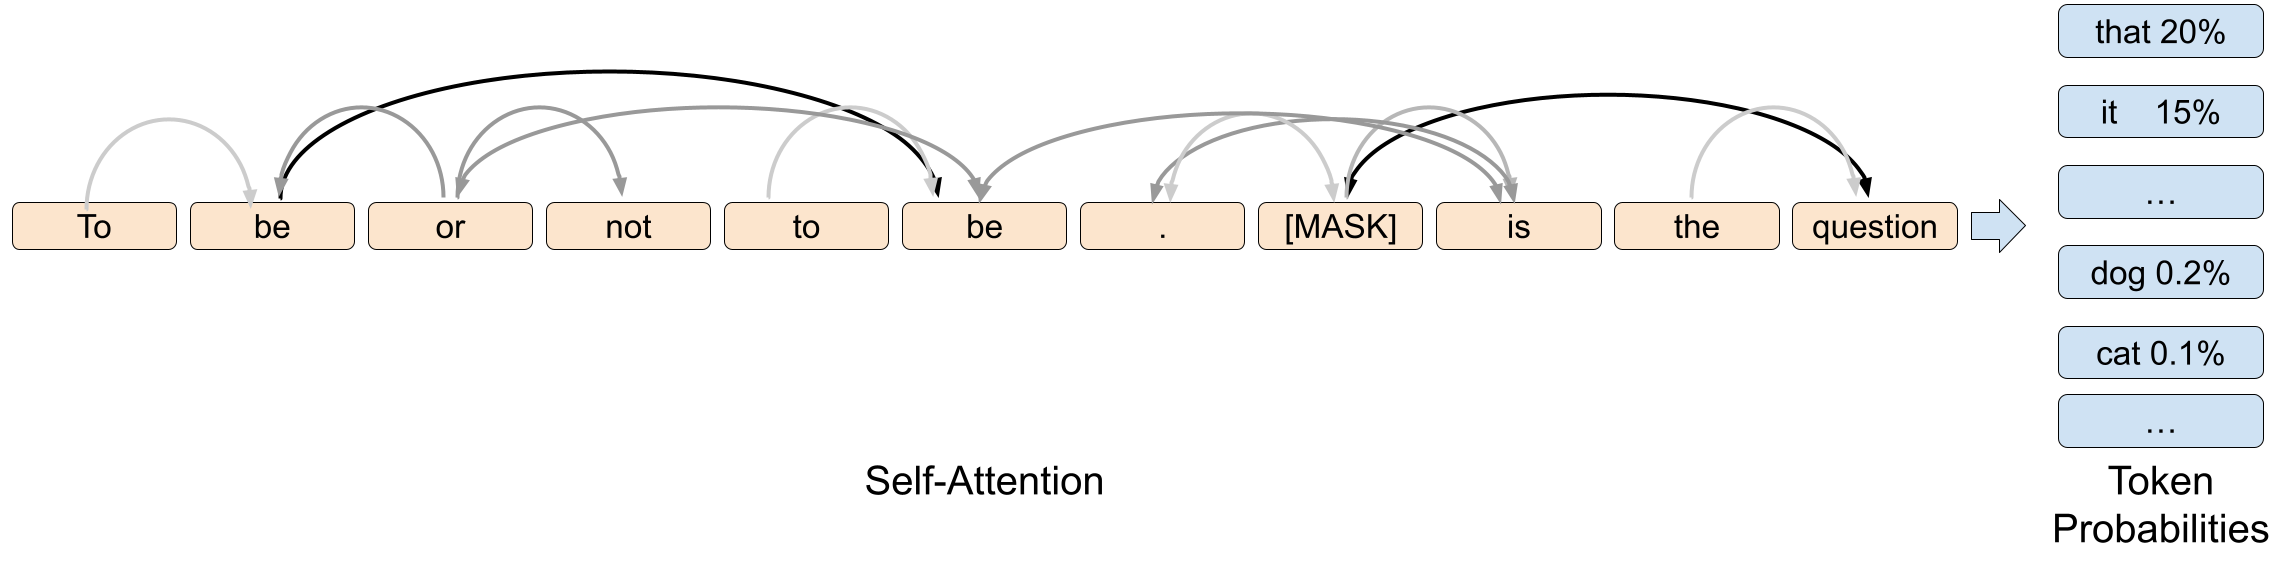
\includegraphics[width=\textwidth]{Figures/02/02_mlm.png}
    \caption{Self-Attention for MLM}
    \label{fig:02_attention_mlm}
\end{figure}

\customHeader{3}{Next Sentence Prediction}
\label{02_next_sentence_prediction}


To learn embeddings for sentences, the Next Sentence Prediction task used by the authors involves joining two sentences or phrases and training the model to determine if they appeared consecutively in the training dataset. 
Specifically, for each example with sentences $A$ and $B$, there's a 50\% chance that $B$ is the actual subsequent sentence to $A$, and a 50\% chance it's a random sentence from the dataset. 
In order to do this, the authors introduce two special tokens, the \texttt{[CLS]} token, for classification, and the \texttt{[SEP]} token to  separate the texts. 

During training, the \texttt{[CLS]} token is placed at the start of the text, and the \texttt{[SEP]} token is positioned between the two sentences. After processing by the encoders, the \texttt{[CLS]} token's embedding undergoes further refinement via a \emph{Pooling Layer}\footnote{This layer comprises a linear layer with a \gls{tanh} activation function}, resulting in what's termed the aggregated or \emph{pooled} output. This pooled output aims to encapsulate the entire text's meaning. Ultimately, this output is fed into a classification layer, and the generated probabilities are matched against the known sentence distribution to compute the cross-entropy (as illustrated in Figure \ref{02_next_sentence_prediction}). Through this process, \gls{bert} is trained to generate embeddings that represent whole sentences.



\begin{figure}
  \makebox[\textwidth][c]{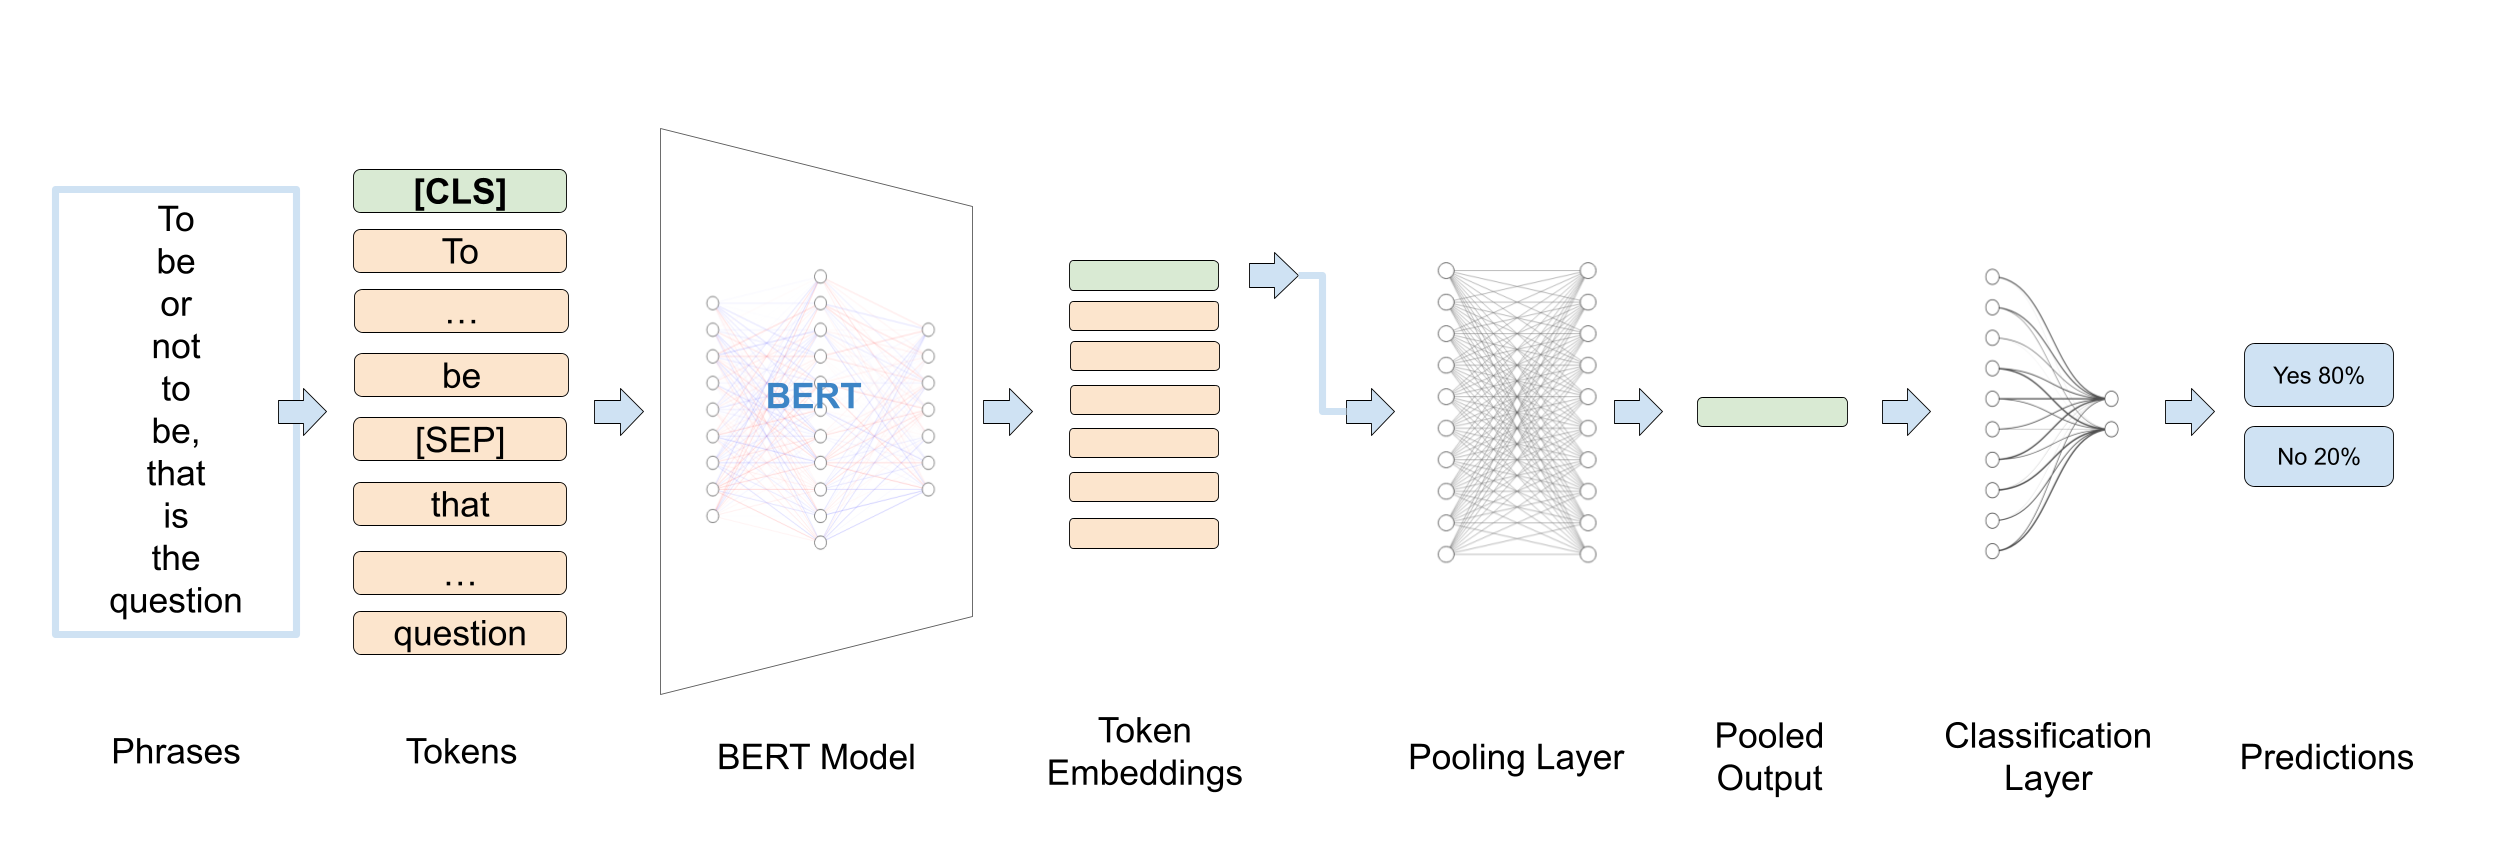
\includegraphics[width=0.9\paperwidth]{Figures/02/02_next_sentence_prediction.png}}%
  \caption{Next Sentence Prediction Task for \BERT{}}
  \label{fig:02_next_sentence_prediction}
\end{figure}



\customHeader{2}{Using \BERT{} for \textclassification{}}
\label{02_using_bert_for_text_classification}


The training process for \gls{bert} doesn't require the texts to be labeled or categorized, making it an \emph{unsupervised} approach. This approach allowed \gls{bert} to learn general text representations that encompass a variety of syntactic and semantic patterns across diverse contexts.

\putInBox{
Once the \gls{bert} model is trained, the conventional method for Document Classification using \gls{bert} involves feeding the text to the model\footnote{keeping the second sentence empty after the \texttt{[SEP]} token}. Then, the pooled output serves as the document's embedding. This embedding is then fed to a classification layer, which is further trained for the specific task at hand (as illustrated in Figure \ref{fig:02_bert_for_document_classification}).
}


\begin{figure}
    \centering
    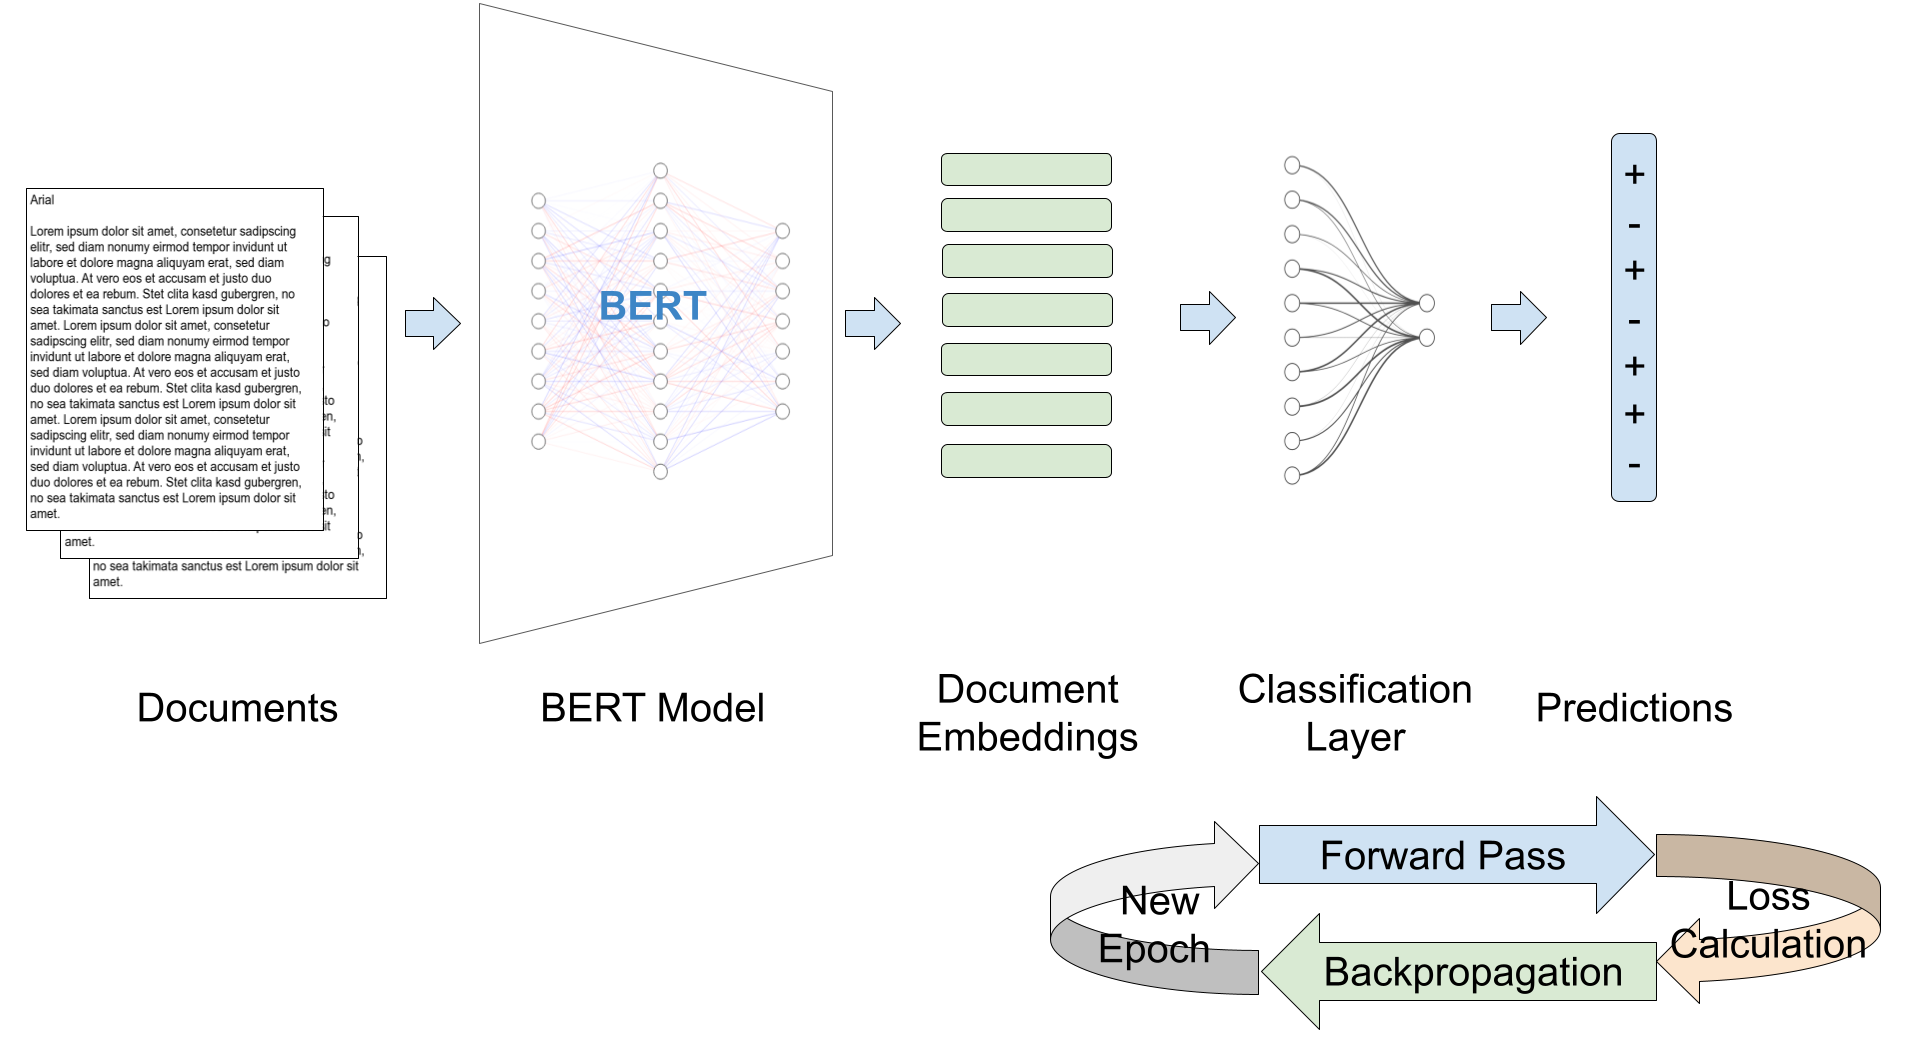
\includegraphics[width=\textwidth]{Figures/02/02_BERT_for_document_classification.png}
    \caption{Using \BERT{} Embeddings for Document Classification}
    \label{fig:02_bert_for_document_classification}
\end{figure}




% Self Attention
% Training
% MLM, next sentence prediction

% input size, attention heads, layers, 
% CLS, pooled output


